%! Author = angela
%! Date = 24/01/24
% !TeX root = ../thesis-main.tex

%----------------------------------------------------------------------------------------
\chapter{Introduction}
\label{ch:introduction}
%----------------------------------------------------------------------------------------
\section{Context}
\label{sec:context}

Computing devices are becoming cheaper and more \emph{ubiquitous}, increasing the complexity of distributed systems.
It is now common for individuals to own multiple computing devices of varying types,
resulting in technology becoming more integrated into daily activities.
Hence, the need to engineer and coordinate the operations in such systems, one way is to program and operate in terms of
    \emph{aggregates} devices, rather than manage each single device.
In actual fact, the coordination of macroscopic behavior in collective systems through a single program is a form of
~\emph{macroprogramming}.
However, this approach presents some primary challenges such as ensuring resilience, efficiency and privacy.

\paragraph{Macroprogramming}
?
%Macroprogramming: Concepts, State of the Art, and Opportunities of Macroscopic Behaviour Modelling
%todo

\paragraph{Self-Organisation}
Coordination modes are based on the notion that interactions among multiple independent and autonomous software systems
can be designed as a space orthogonal to pure computation.
This idea can be reified into a concept of shared data space, enabling so-called \emph{generative communication}.
%Todo talk about Linda and Mars ???
Over the course of time, different approaches have been created, such as \emph{Linda} and \emph{Mars},
suggesting innovative techniques for programming systems with devices of different nature focusing on the coordination
of centralised local components, but not on the distribution of the systems.
The main problems that can be encountered in distributed systems are dealing with
    i) openness, as unexpected environment changes,
    ii) large scale of agents and coordination abstractions to be managed,
    iii) intrinsic adaptiveness, such as the ability to intercept relevant events and react to them, guaranteeing
        the resilience of the system.
The challenges necessitate a \emph{self-organising coordination} approach, wherein coordination abstractions solely
manage logical interactions.
This ensures the emergence of global and robust patterns of correct coordination behaviour.


\subsection{Computational Fields}
\label{subsec:computational-fields}
%todo cite From distributed coordination to field calculus and aggregate computing

\paragraph{Field-Based Coordination}
To facilitate self-organisation patterns of agents in complex environments, the concept of \emph{coordination field}
has been introduced.
This abstraction serves as a navigational tool for agents over the actual environment.
%todo cite tota
In this context, the tuple-based middleware TOTA (Tuples On The Air) has been suggested to support field-based
coordination for pervasive-computing applications.
Initially, each field of the tuple in the system was assigned a name, along with a formula that supports the
if-then-else construct and includes arithmetic and boolean operators to specify the field's behaviour over time.
Secondly, it was introduced an operator in the tuple space responsible for applying formulas using contextual information.\\
Somewhat independently of the challenge of identifying appropriate coordination models for distributed and situated systems,
several studies have tackled analogous issues in the broader endeavour of constructing distributed intelligent systems.
This involves promoting higher abstractions of spatial collective adaptive systems.

\paragraph{Field Calculus}
Among the studies such as for managing space-time computing models for the manipulation of distributed data structures,
the notion of \emph{computational fields} were proposed.
Consequently, the ~\ac{fc} has been proposed as a foundational model for the coordination of computational
devices spread in physical environments, also known as \emph{aggregate computing}.
%todo is it necessary to insert the abstract syntax of the field calculus?
~\ac{fc} was introduced as minimal core calculus with the aim of capturing the fundaments that make use of computational
fields: functions over and with fields, their evolution over time and the construction of field of values from neighbours.

The main concept of \ac{fc} is to specify the aggregate system behaviour of a network of devices, where devices that can
directly communicate with each other are indicated through a dynamic network relation.
An example of its application is within a sensor network with a range of a broadcast communication.
The behaviour is applied through a functional composition of operators that manipulate the computational fields,
called specification, that can be interpreted locally or globally.
A local specification can describe a computation on an individual device executed in asynchronous ``computation rounds'',
including sending or receiving messages from neighbours, getting information from sensors and computing the local value of the field.
In the global view, a field calculus expression specifies a mapping associating each computation round of each device to
the value that it assumes at that space-time event.
This dual nature inherently facilitates the alignment of individual device behaviour with the overarching global behaviour
of the entire network of devices.

%rep(e_1)\{(x)=>e_2\}
%if(e_0)\{e_1\}\{e_2\}
\paragraph{Syntax of field calculus}
The \emph{field calculus} is based on a minimal set of operators.
\begin{itemize}
    \item \emph{Stateful field evolution}: the expression \lstinline|rep(e_1){(x)=>e_2}| describes a field evolving in time.
        \lstinline{e_1} represents the initial field value, the function \lstinline|(x) => e_2| declares how the field changes
        at each execution;
    \item \emph{Neighbour interaction}: the expression \lstinline|nbr{e}| builds a neighbouring field, a view of the field
        values in the surroundings of each device where neighbours are mapped to their evaluations of \texttt{e};
    \item \emph{Domain partitioning}: the expression \lstinline|if(e_0){e_1}{e_2}| splits the computational field into
        two non-communicating zones hosting isolated computations: \lstinline|e_1| where \lstinline|e_0| is \texttt{true} and
        \lstinline{e_2} where \lstinline{e_0} is \texttt{false} %todo fix pedix
\end{itemize}

\subsection{Aggregate Computing}
\label{subsec:aggregate-computing}
%TODO cite Modelling and simulation of Opportunistic IoT Services with Aggregate Computing

\paragraph{Aggregate programming}
Aggregate programming elaborates a layered architecture that aims to simplify the design, creation and maintenance of
distributed systems.
Through this methodology, the fundamental unit of computation shifts from an individual device to a collaborative
ensemble of devices.
It elaborates a layered architecture that aims to simplify the design, creation and maintenance of complex distributed
systems.
Moreover, aggregate programming provides mechanisms for robust and adaptive coordination through simple programming APIs
that implicitly guarantee safety and resilience.
This framework is useful in large-scale scenarios, where there is insufficient fixed network infrastructure, as seen in
situations like crowd management during large public events.

%todo mention this figure somewhere
\begin{figure} %[!ht]
    \centering
    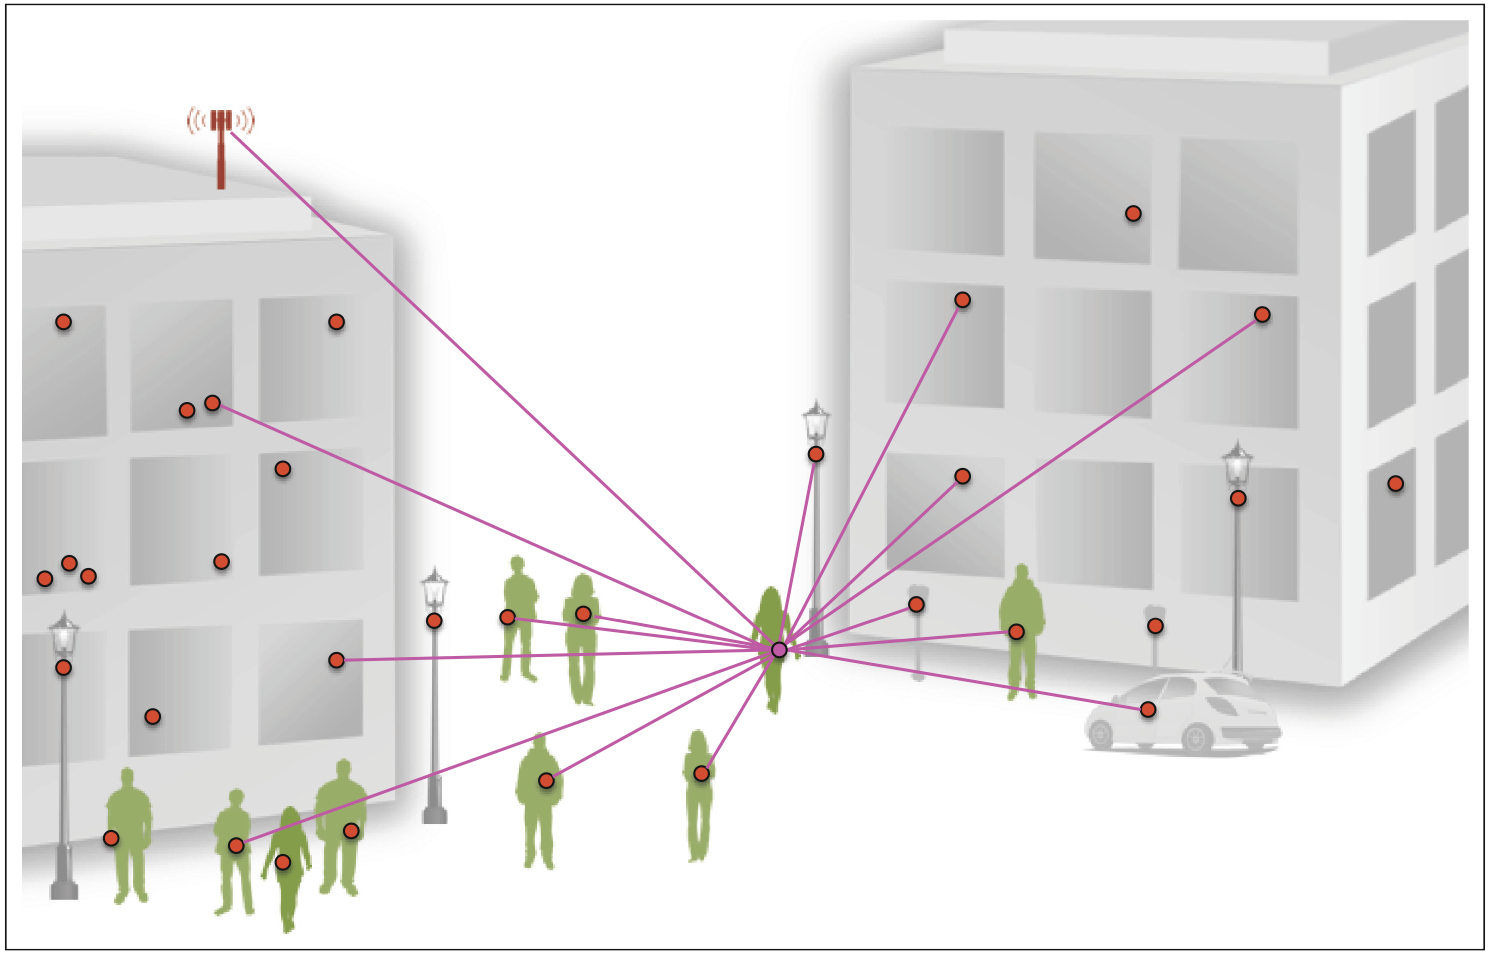
\includegraphics[width=.8\linewidth]{figures/smart_network_objects}
    \caption{Our world is increasingly populated with a wide range of computing devices, embedded in our environment
    and with many opportunities for local and even location-indipendent interactions on fixed network infrastructures.}
    \label{fig:smart-network-objects}
\end{figure}

In various environments, interactions between wearable devices such as smartphones can support different kinds of services,
including crowd detection, crowd-aware navigation or dispersal advice.

\paragraph{Aggregate computing}
~\ac{ac} is a paradigm and engineering approach for the compositional development of self-adaptive ~\ac{iot} services
from a global perspective.
It has been developed with the core idea of functionality composing collective behaviours to achieve effective and resilient
complex behaviours in dynamic networks.
It views a given environment as a whole programmable entity whose parts collaboratively produce and consume services
across space and time.
~\ac{ac} is based on the principles of~\ac{fc} that is a functional programming model used to specify
and compose collective behaviours with formally equivalent local and aggregate semantics.
The concept of \emph{computational fields} can be viewed as a distributed data structure,
with the aim of conceptually mapping each device to a value produced in a program, considering both
space and time.
Therefore, its structure supports the specification, analysis, simulation and runtime execution of \emph{collective}
or \emph{aggregate} services, independently of the specific~\ac{iot} architecture.

This paradigm has three key traits that characterise it:
    i) \emph{Global stance with global-to-local mapping}, where the target of system design is the entire distributed
        \ac{iot} ecosystem,
    ii) \emph{Behaviour compositionality}, whereby a rich collective service can be described in terms of the functional
        composition of simpler collective services, and
    iii) \emph{Abstraction}, by which aggregate services enable adaptivity at different levels by abstracting from low-level
        issues and details.
These attributes are crucial both in the design phase, where intricate solutions can frequently be articulated concisely
and declaratively, and in the operational phase, where considerable flexibility is granted to the devops team and the
platform regarding execution specifics and deployment strategies.

\paragraph{Software platforms}
~\ac{ac} is designed to address many application scenarios, typically characterised by inherent distribution, heterogeneity,
mobility and a lack of stable infrastructure.
There are various strategies by which an~\ac{ac} system can run, contingent upon the selected and implemented
communication methodologies.
Programs can be executed within a fully distributed peer-to-peer environment, where end devices communicate directly
with peer neighbours, and each independently runs its fragment of aggregate logic.
On the opposite side, there are entirely centralised solutions, where end devices function solely as manager for sensors
and actuators, forwarding perceptions upstream to one or more servers.
These servers perform computations on behalf of the devices and subsequently transmit actuation data downstream.
Thanks to this flexibility of its applications,~\ac{ac} has the potential to facilitate the creation of a more systematic
spectrum for transitioning between cloud and distributed systems.
This approach also embraces the emerging domains of edge and fog computing.
%todo talk about edge e fog computing??

\paragraph{Aggregate computing in adaptive \ac{iot} Services}
Thanks to its features, \emph{aggregate computing} is well suited for the development of \emph{Opportunistic \ac{iot}
Services}, supporting the properties:
\begin{itemize}
    \item \emph{Dynamicity}: the direct support for opportunistic service activation and evolution is achieved through
        code mobility and constructs that define dynamic domains of computations dependent on space and time;
    \item \emph{Context-awareness}: aggregate programs utilize sensors, communication driven by neighborhood interactions,
        and iterative execution to consistently evolve the set of local contexts.
        This evolution forms the basis for the unfolding of computation and coordination logic;
    \item \emph{Co-location}: as a natural method to define the concept of neighbourhood, relies on a physical space basis.
        \ac{ac} inherently incorporates locality (both in space/time and purpose) to organise interactions and activities;
    \item \emph{Transience}: \ac{ac} provides constructs that directly supports the execution of distributed services
        based on time and context awareness.
\end{itemize}

\paragraph{Computational model}
%todo I can see this as ubiquitous language
There are some concepts and relationships included in the \emph{aggregate computing} context:
\begin{itemize}
    \item \emph{Aggregate program}: an executable representation of specific aggregate logic that defines a collective behaviour;
    \item \emph{Aggregate system}: a set of interconnected nodes or devices that support the collective execution of aggregate programs;
    \item \emph{Aggregate application}: a specific aggregate logic operating on a designated aggregate system, aimed at
        solving particular problems in a specific context;
    \item \emph{Node}: also referred to as \emph{device}, it represents an individual \ac{ac}-enabled entity, potentially
        equipped with sensors and actuators;
    \item \emph{Neighbourhood}: the logical or physical set of nodes that can be directly contacted by a given node;
    \item \emph{Global or local sensor}: a source for global or local information;
    \item \emph{Global or local actuator}: a global or local actionable device for environment-directed actions;
    \item \emph{Global or local computational environment}: anything that is detectable and subject to action through the
        use of global (or local) sensors and actuators
        This also includes the shared functionalities offered by the platform.
\end{itemize}

The networked devices inside an aggregate system compute and communicate at asynchronous rounds of execution.
Each round, each device executes the global aggregate program according to the local semantics; then it updates its internal
state and lastly generates the data for the external communication.
The round is performed by taking into account the computational context created by the previous state, sensor data and
messages from neighbouring devices.
After the execution of the round, result data are made available to neighbours and eventually instructed actuations are
locally executed.
The system can continuously react to changes by repeatedly executing rounds, allowing for self-adaptation to contextual changes.

\paragraph{Models alignment}
Due to the high-level and platform-independent metamodels of \ac{iot} and \ac{ac} systems, each with different goals or
abstraction levels, it is necessary to align the two metamodels.
This ensures that their unique focus is taken into account.
There are some main differences between the two metamodels:
\begin{itemize}
    \item the concept of device is different, for \ac{ac} is logical and is not the same as a device component of a Smart Object;
    \item although ensembles of Smart Objects are conceptualised as firs-class concept in \ac{ac}, they are not explicitly
        represented in the \ac{iot} system metamodel;
    \item the concept of neighbourhood in \ac{ac} regulates local, contextual communication among its devices.
        However, this concept cannot be explicitly mapped to \ac{iot} system concepts because device-to-device relationships
        are abstracted away from the metamodel.
\end{itemize}

\subsection{XC}
\label{subsec:xc}
\textbf{XC} is an experimental programming language design to develop \emph{homogeneous} distributed systems.
Those kinds of systems consist of similar devices that communicate to neighbours and execute the same program.
The aim of this experimental language is to push the abstraction boundaries farther than actual existing approaches.
Many issues can arise in distributed systems, like concurrency, remote communication, asynchronous execution, message
loss, and device failures.
These kinds of problems must be taken into account when designing a programming language for such systems.
Some of the possible applications of this approach may be crowd management, gossip-based data aggreation, task allocation
in robot swarms and coordination of enterprise servers. %todo add cites that are in the xc paper
The homogeneity in large-scale systems also arises when each device executes a program from a predefined set, reflecting
a homogeneous configuration featuring a single program with an initial branch.

%This design eliminates the need to handle the aforementioned problems explicitly.
%Additionally, distributed programs with independent devices retain composability through a mechanism called \emph{alignment}.

\paragraph{System model}
Devices that can send or receive messages are called \emph{neighbours}, and they can change dynamically to model network
delays, failures or spatial movements.
Based on existing homogeneous systems, the device behaviour has been abstracted through a notion of \emph{execution round},
in which a device independently executes an \textbf{XC} program and sends the resulting messages to its neighbours.
Referring to \emph{macroprogramming}, each device's behaviour in the network is developed as a single program, with no
assumption of when an execution round will occur, meaning that they are entirely asynchronous.

Messages are handled queueing up in a buffer; when a device executes its \textbf{XC} program, it processes the received
messages producing others to send to neighbours, that in turn will process their messages.
%todo insert graph of the system model

It can occur that a device executes multiple rounds before a neighbour executes its own, in that case the neighbour will
only see the last received message from the first device; newly received messages will overwrite the older ones.
Messages can persist across rounds; they are not removed from the buffer after they have been read unless they expire.
The devices for which a message is available in a certain round are considered the \emph{neighbours} for that round.

\paragraph{Data types}



\paragraph{Alignment}
The \emph{alignment} is a mechanism that enables developers to abstract over asynchronous execution while still retaining
composability.

\section{Motivations}
\label{sec:motivations}

%vantaggi > benefits/utility

\subsection{Heterogeneity limitations}
\label{subsec:heterogeneity-limitations}

\subsection{Goal}
\label{subsec:goal}


\section{State of Art}
\label{sec:state-of-art}

\subsection{Protelis}
\label{subsec:protelis}

\subsection{ScaFi}
\label{subsec:scafi}

\subsection{FCPP}
\label{subsec:fcpp}


%
%Write your intro here.
%\sidenote{Add sidenotes in this way. They are named after the author of the thesis}
%
%You can use acronyms that your defined previously,
%such as \ac{IoT}.
%%
%If you use acronyms twice,
%they will be written in full only once
%(indeed, you can mention the \ac{IoT} now without it being fully explained).
%%
%In some cases, you may need a plural form of the acronym.
%%
%For instance,
%that you are discussing \acp{vm},
%you may need both \ac{vm} and \acp{vm}.
%
%\paragraph{Structure of the Thesis}
%
%\note{At the end, describe the structure of the paper}
%
